\documentclass[8pt]{beamer}

\usetheme[progressbar=frametitle]{metropolis}
\usepackage{booktabs}
\usepackage[scale=2]{ccicons}
\usepackage[utf8]{inputenc}
\usepackage{ragged2e}
\usepackage{pgfplots}
\usepgfplotslibrary{dateplot}
\usepackage{xspace}
\newcommand{\themename}{\textbf{\textsc{metropolis}}\xspace}

\title{\textbf{\huge{CMS at LHC}}}

\date{\today}
\author{\textbf{Diego Barón}}
\institute{Universidad de Antioquia, Instutito de Física.}

\begin{document}

\maketitle

\begin{frame}{Table of contents}
  \setbeamertemplate{section in toc}[sections numbered]
  \tableofcontents[hideallsubsections]
\end{frame}


\section{Motivation.}

\begin{frame}[fragile]{Motivation}

Particle physics experiments can be done studying cosmic rays, solar neutrinos, dark matter in galaxies, etc. 

\begin{exampleblock}{But don't forget accelerators... }
This experiments are the most popular because we can control almost all the initial conditions:
\begin{itemize}
\item The particles involved.
\item The energy of the beams.
\item The geometry of the experiment
\item The amount of particles. 
\end{itemize}    
\end{exampleblock}

Experimental particle physicists must know and understand how experiments works in order to know:
\begin{itemize}
\item What to look for.
\item And how to.
\end{itemize}

\end{frame}

\section{The problem.}
\begin{frame}[fragile]{The problem.}
\centering
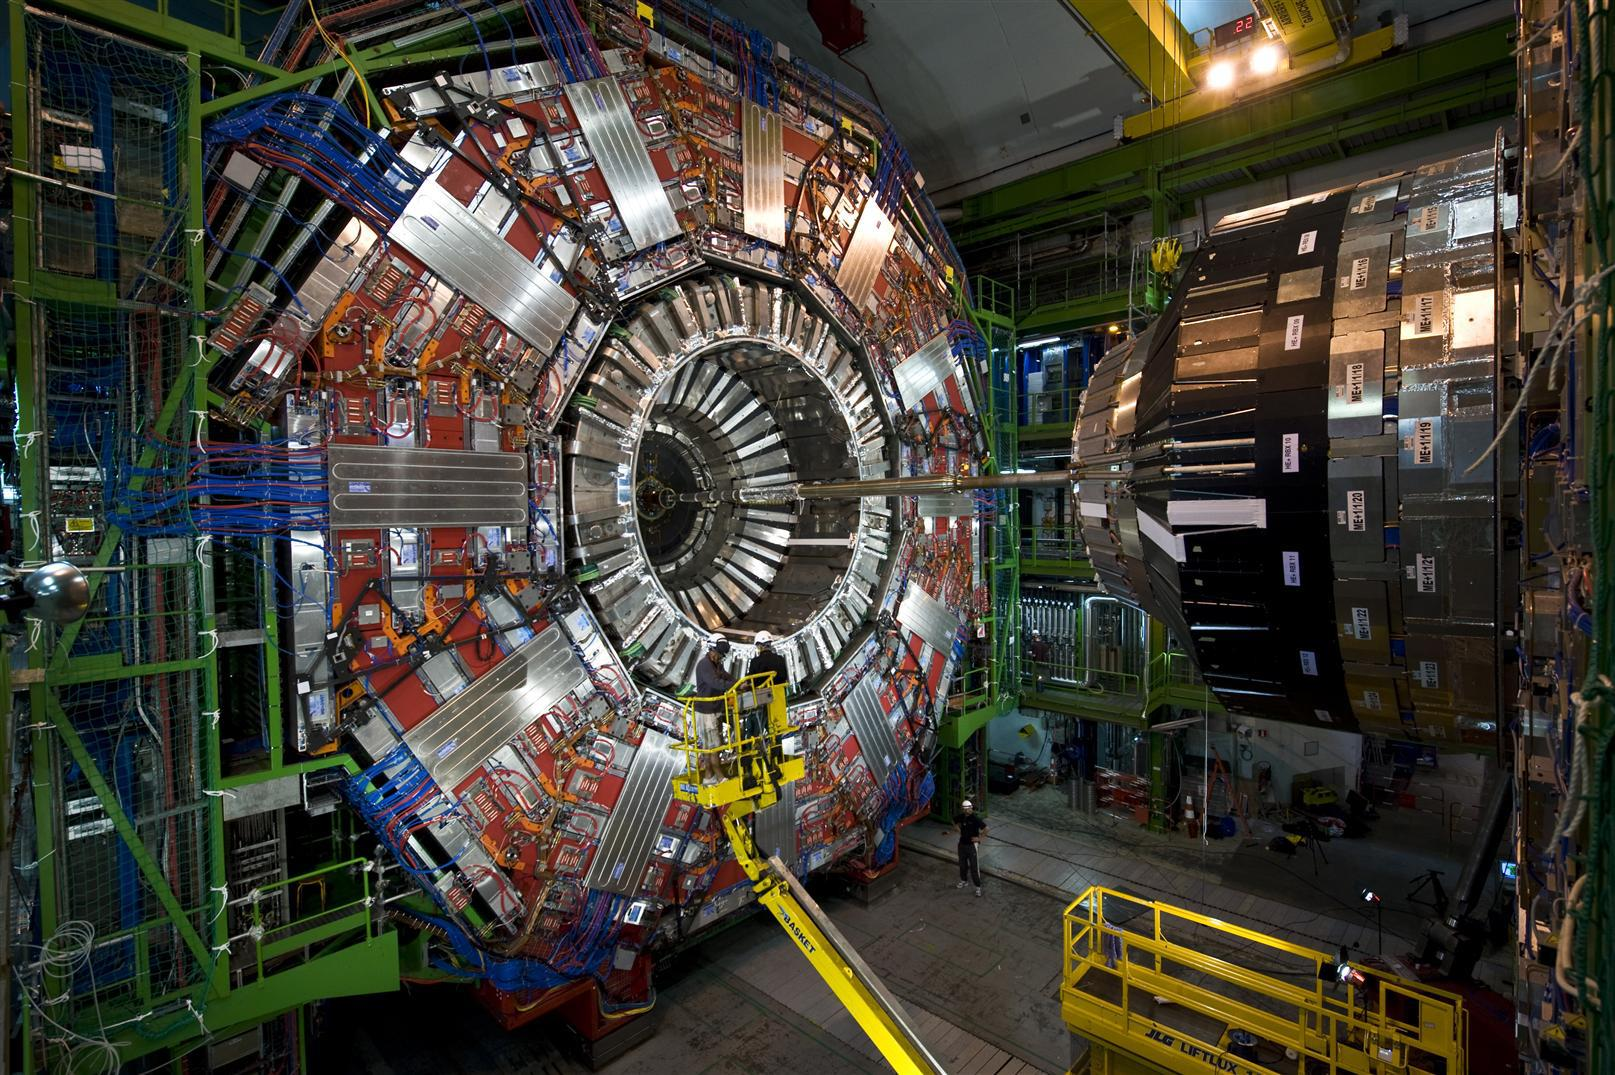
\includegraphics[height=7cm,width=9cm]{1}
\metroset{block=fill}
\begin{exampleblock}{\centering The question is...}
\centering
¿How does CMS at LHC works?

\end{exampleblock}


\end{frame}

\section{First LHC.}

% HHHHHHHHHHHHHHHHHHHHHHHHHHHHHHHHHHHHHHHHHHHHHHHHHHHHHHHHHHHHHHHHH

\begin{frame}[fragile]{LHC.}
Is the main accelerator managed by CERN (European Organization for Nuclear Research). 
21 member states-113 participant countries.

It`s the biggest particle collider on Earth:
\begin{itemize}
	\item 27 km circunference.
	\item 14 TeV at the center of mass. (8 TeV reached at Run 1)
	\item 100 m under the ground.
	\item 4 main experiments (detectors): ALICE,CMS,ATLAS,LHCb
\end{itemize}
The two principal parts are the injector chain and the main ring.
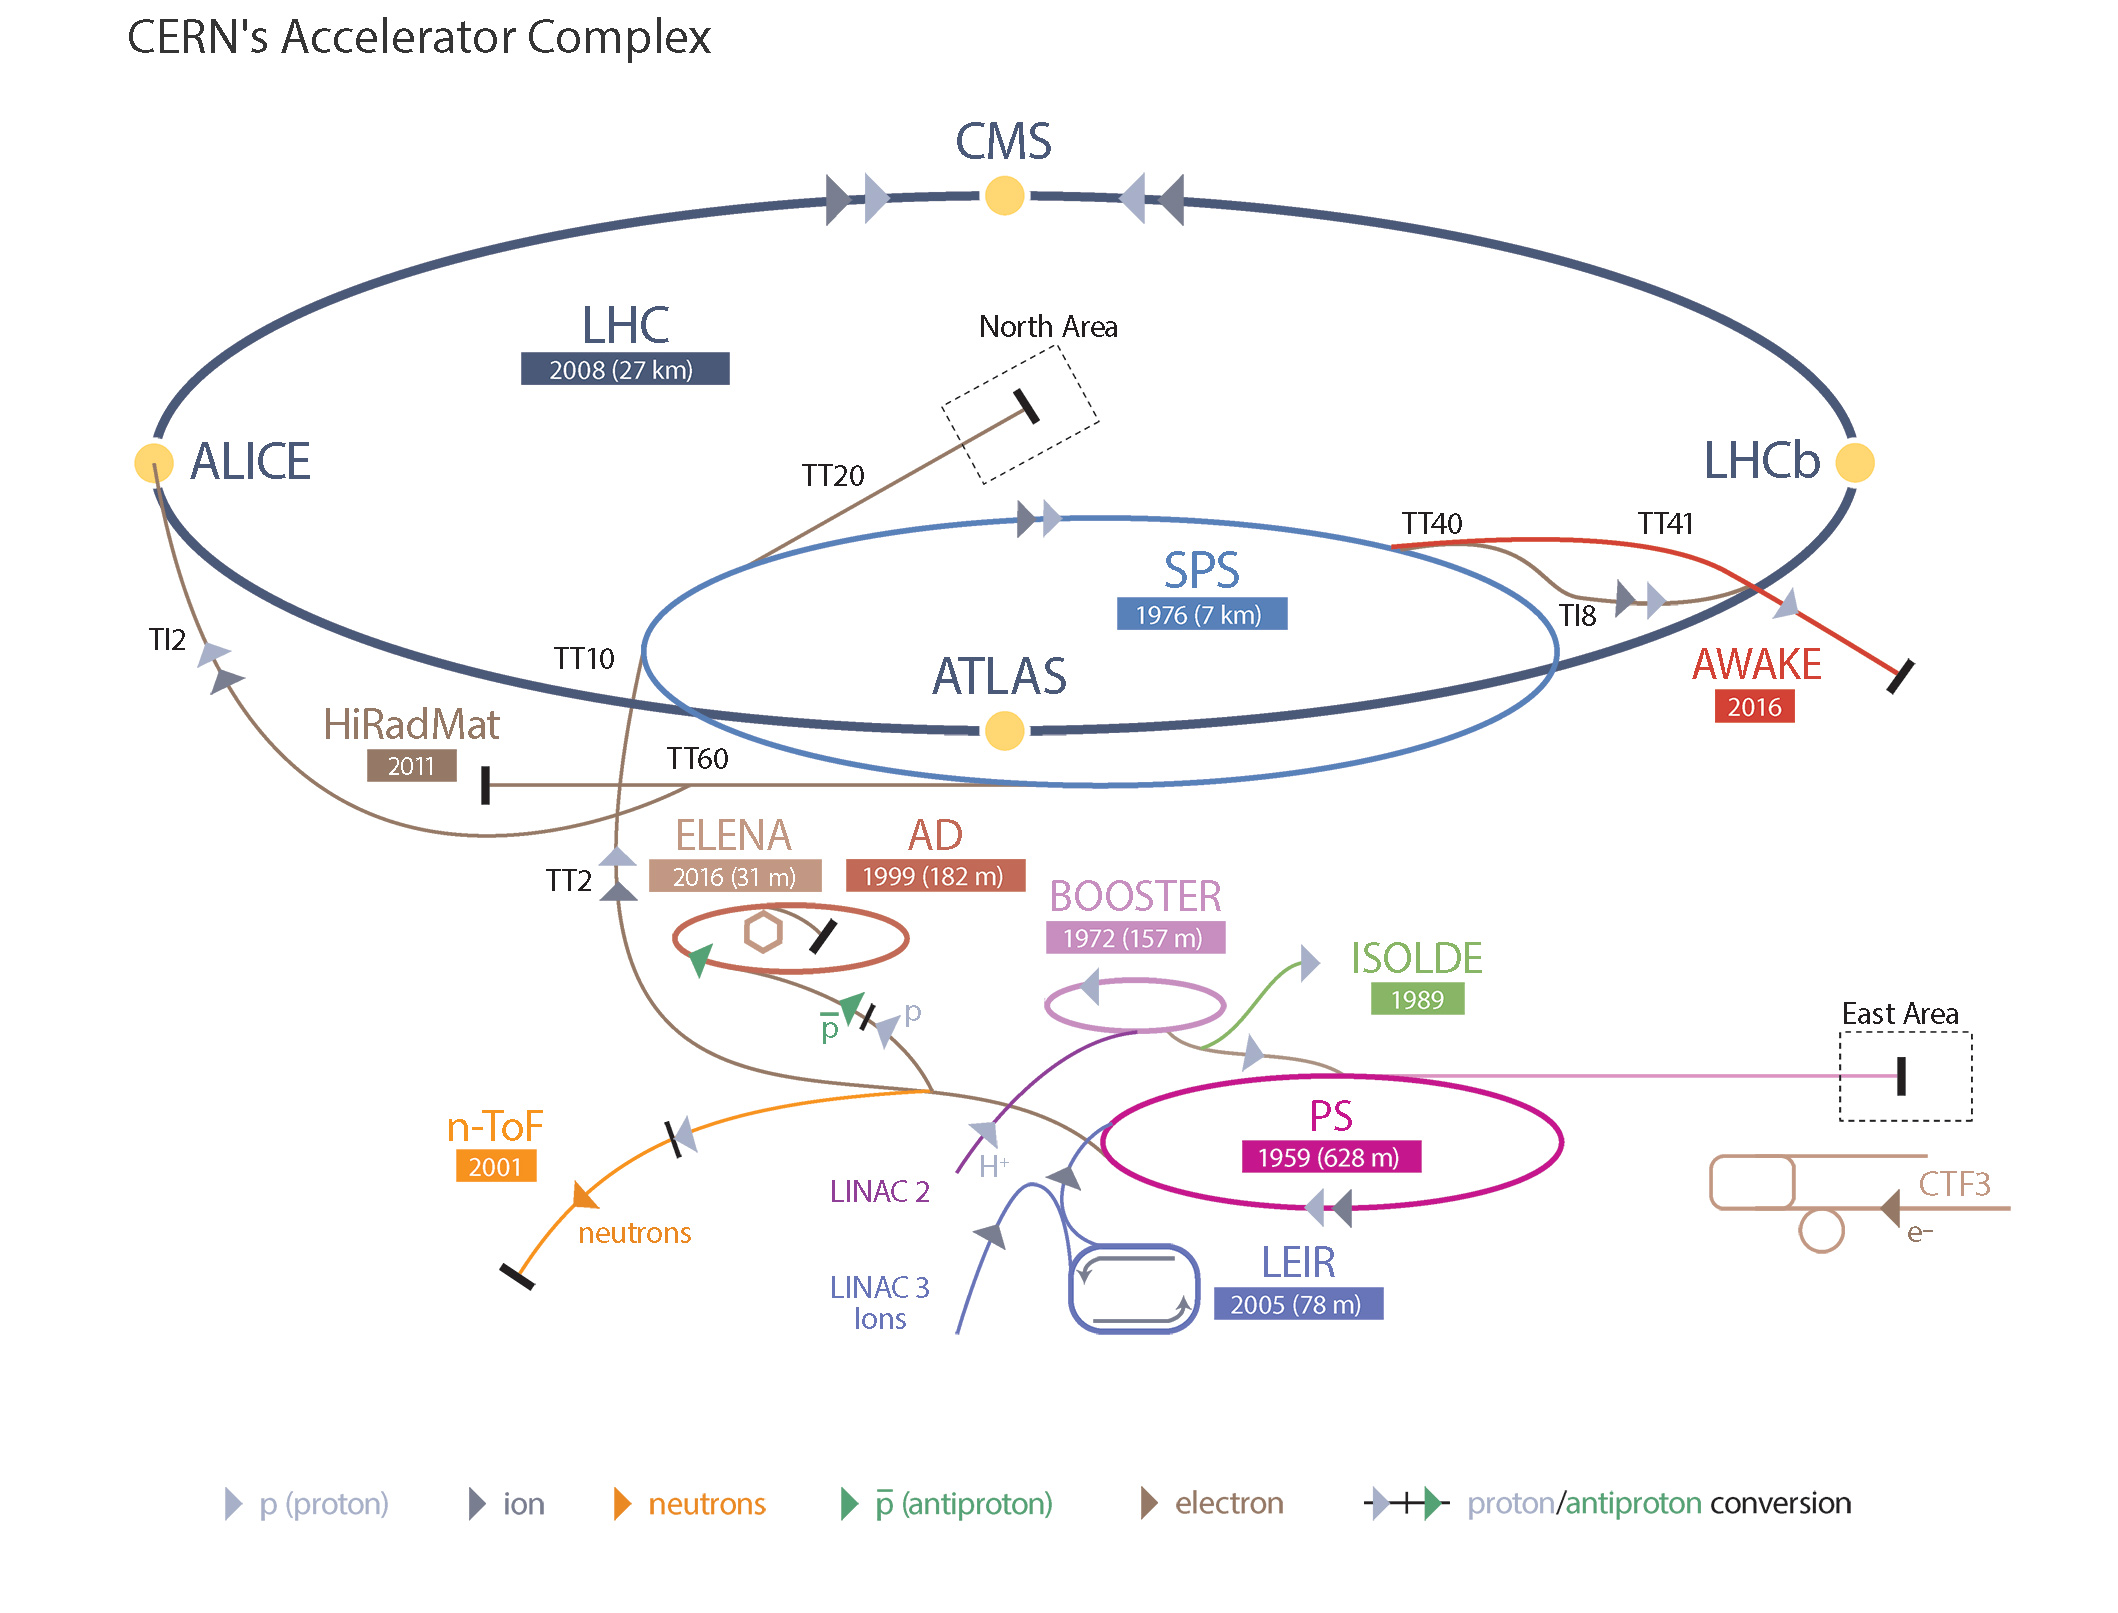
\includegraphics[height=5cm,width=10cm]{2}
\end{frame}

% HHHHHHHHHHHHHHHHHHHHHHHHHHHHHHHHHHHHHHHHHHHHHHHHHHHHHHHHHHHHHHHHH

\begin{frame}[fragile]{The injector chain.}
Before reaching main ring, protons pass by a series of stages:
	\begin{itemize}
		\item Extracted via ionization of Hydrogen in the Duoplasmatron Proton Ion Source.
		\item Accelerated at 50 MeV in Linac2 (1978).
		\item  Linac2 injects protons in the Proton Synchrotron Booster (PSB)
		and are accelerated up to 1.4 GeV.
		\item From PSB, protons are delivered to the Proton Synchrotron (PS) where
		they reach 28 GeV. They are also split from 6 initial bunches to 72, spaced by 25 ns.
		\item  Finally, the pre-acceleration chain is finished by the SPS, the Super Proton Synchrotron. There, the bunches are accelerated up to 450 GeV.
	\end{itemize}
	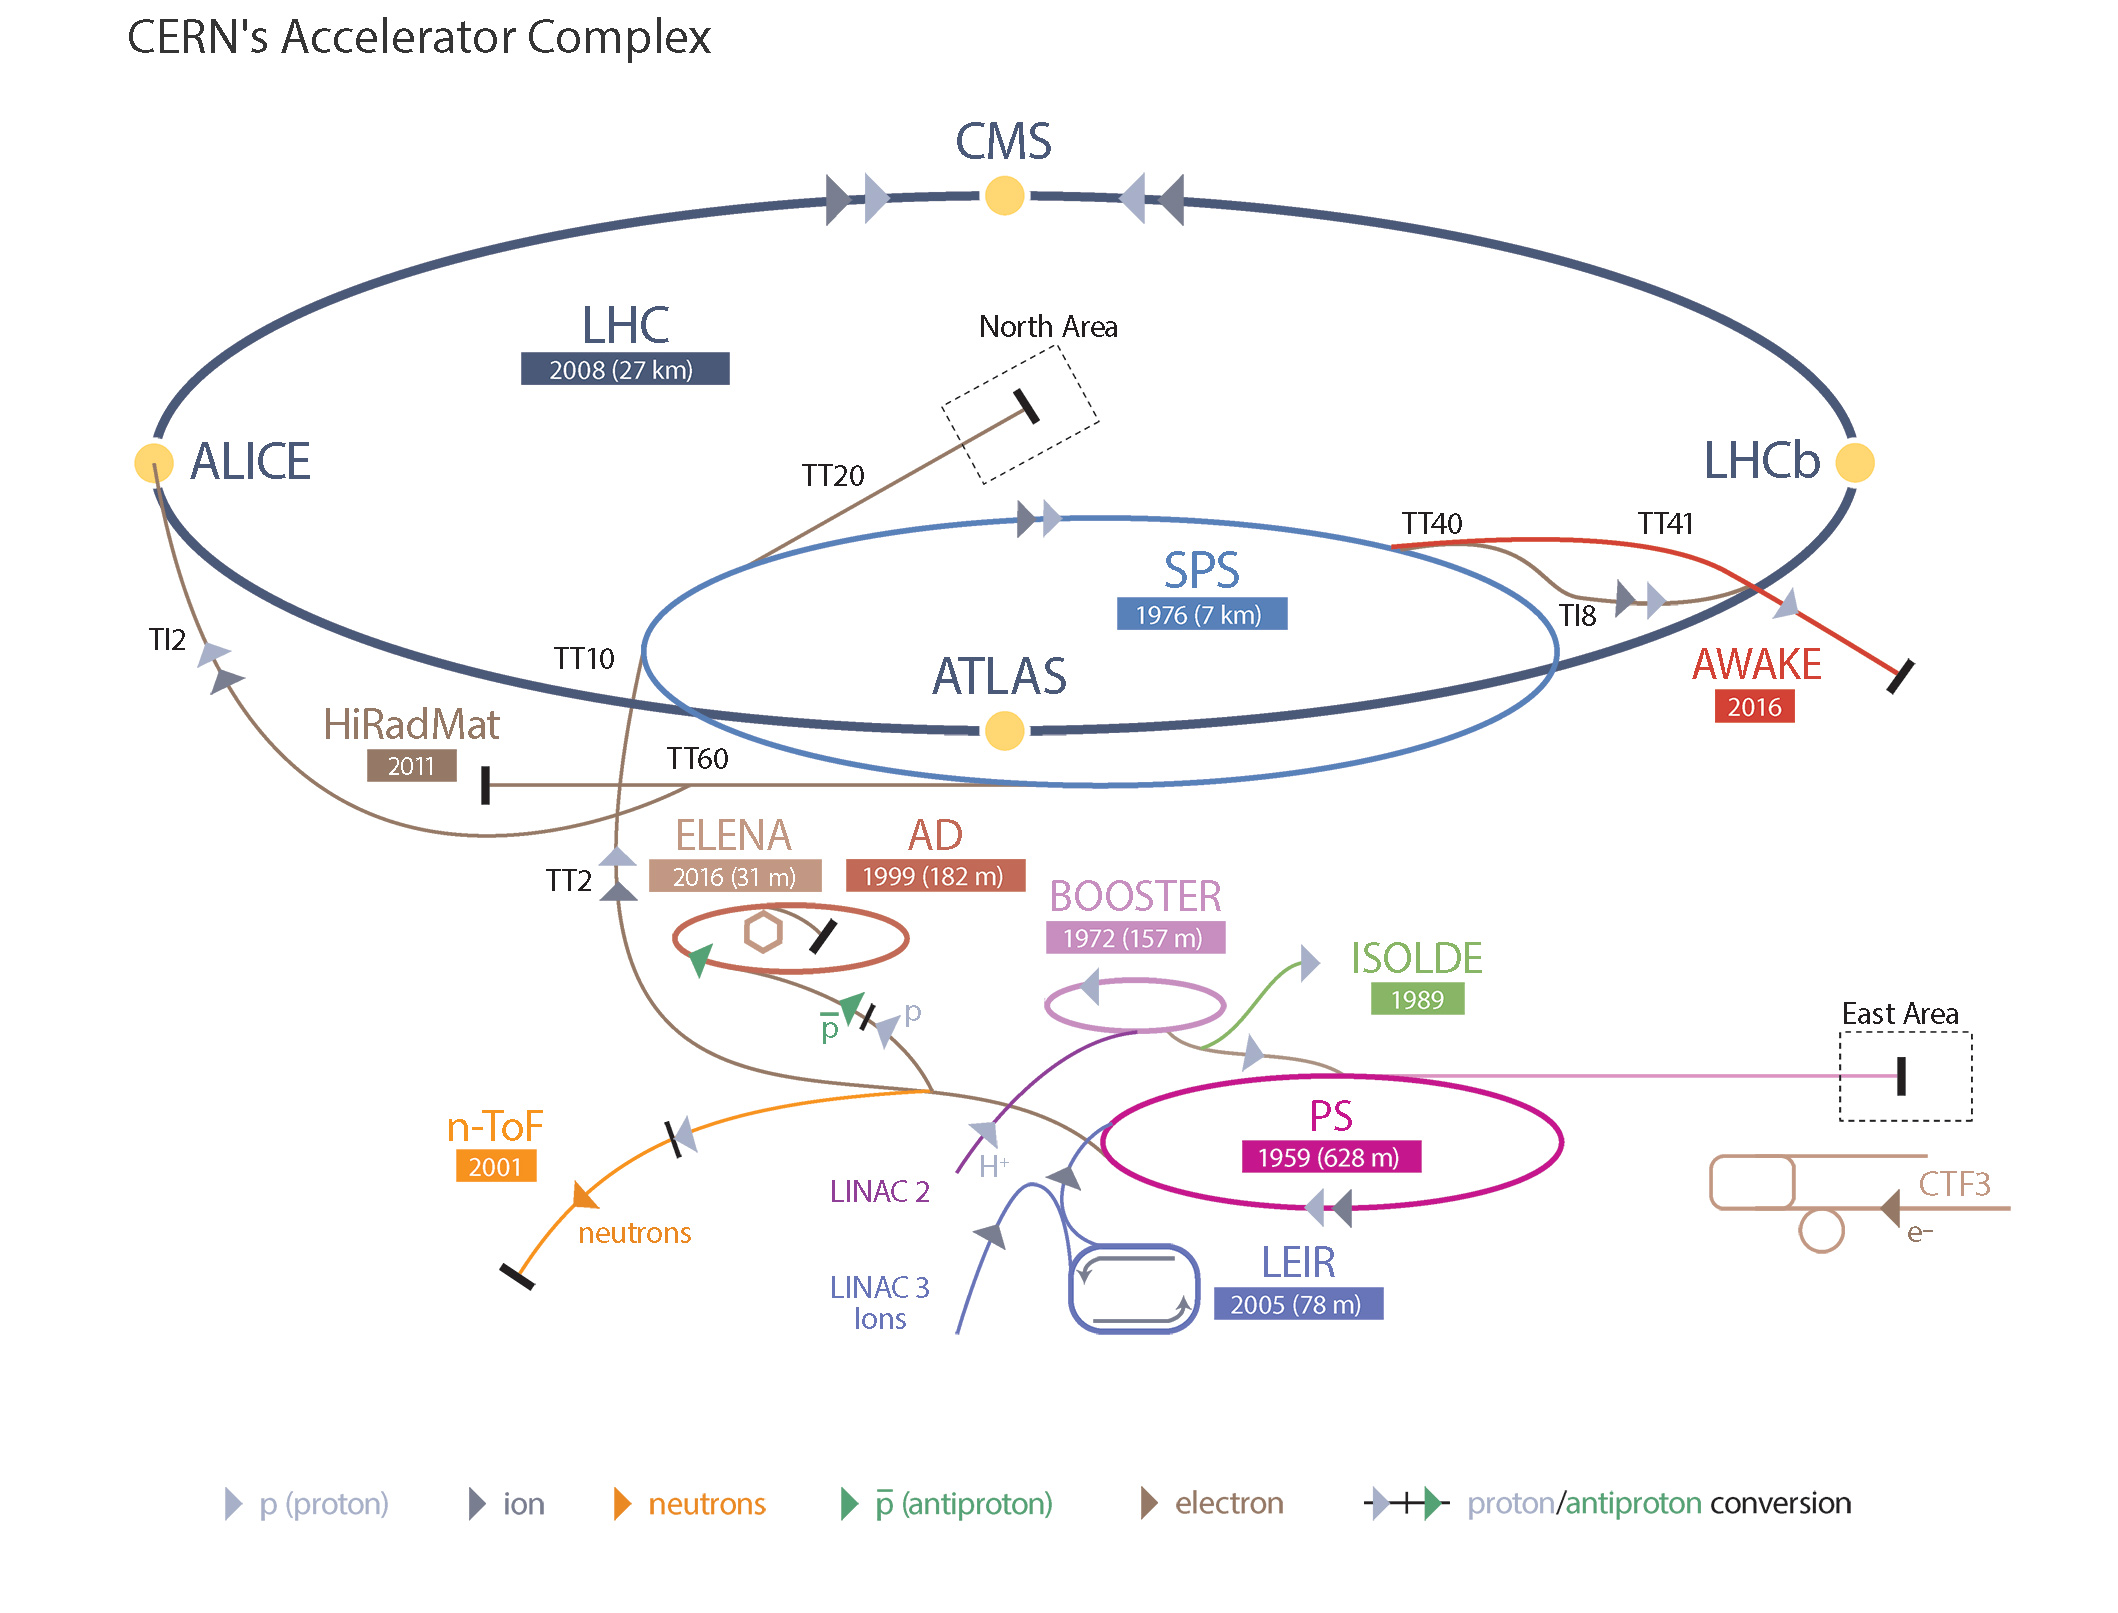
\includegraphics[height=5cm,width=10cm]{2}
\end{frame}

% HHHHHHHHHHHHHHHHHHHHHHHHHHHHHHHHHHHHHHHHHHHHHHHHHHHHHHHHHHHHHHHHH

\begin{frame}[fragile]{LHC main ring.}
	It's composed of two rings that accelerate the proton bunches in opposite directions. Some characteristics of the design are:
	\begin{itemize}
		\item 15m magnets with an strong magnetic field of 8,33T. 
		\item Superconductivity involved (1.9 K).
		\item Ultra high vacuum of $10^{-9}$mbar.
		\item In addition LHC has other magnets to correct different characteristics of the beams: 520 quadrupoles, 2464 sextupoles, 1232 octupoles.
	\end{itemize}
	
	\begin{figure}[!tbp]
		\centering
		\begin{minipage}[b]{0.4\textwidth}
			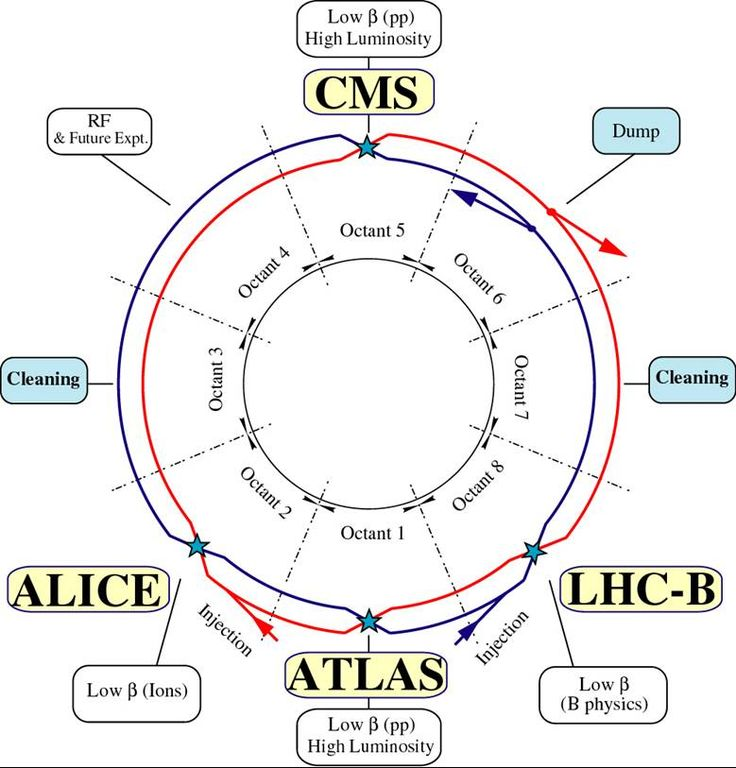
\includegraphics[width=\textwidth]{3}
			
		\end{minipage}
		\hfill
		\begin{minipage}[b]{0.4\textwidth}
			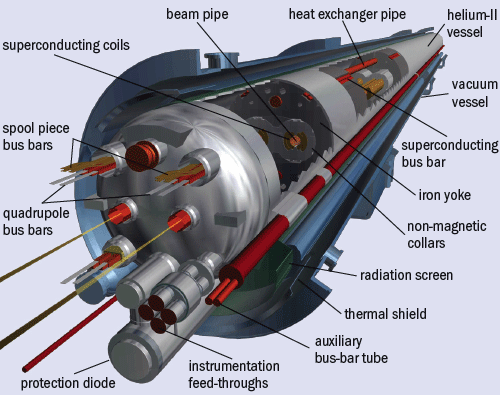
\includegraphics[width=\textwidth]{4}
			
		\end{minipage}
	\end{figure}
\end{frame}

% HHHHHHHHHHHHHHHHHHHHHHHHHHHHHHHHHHHHHHHHHHHHHHHHHHHHHHHHHHHHHHHHH

\begin{frame}[fragile]{LHC main ring.}
	In collider experiments the main character is Luminosity:
\begin{equation}
\nonumber L=\frac{k_nN_{b}^{2}f_{rev}}{4\pi\sigma_x \sigma_y}R
\end{equation}
In LHC design, this parameters have the following values:	
	\begin{table}[]
		\centering
		\label{my-label}
		\begin{tabular}{|l|l|}
			
			\hline
			Energy{[}GeV{]}                                                   &        7000            \\ \hline
			Luminosity{[}$cm^{-2}s^{-1}${]} &      $10^{34}    $           \\ \hline
			$k_b$ Number of bunches                                            &            2808        \\ \hline
			Bunch spacing {[}ns{]}                                            &          24.95          \\ \hline
			$N_b$ intensity per bunch {[}protons/bunch{]}                      &            $1.15\times 10^{11}$        \\ \hline
			$f_{rev}$ revolution frequency {[}kHz{]}                         &           11.25         \\ \hline
			$\sigma_x=\sigma_y$  Beam Standard Deviation  [cm]                    &           7.7         \\ \hline R Geometric reduction factor
			&           0.8         \\ \hline
			
		\end{tabular}
	\end{table}
	Cross section of a proton-proton collision at 14 TeV is 100-110 mb, 3 different processes are involved:
	\begin{itemize}
		\item Elastic scattering: Protons exchange momenta but their structure remains unchanged.
		\item Diffractive scattering: Momenta exchange but additional particles are generated apart from the final protons.
		\item Inelastic scattering: Partons interchange a big amount of momentum and produce several particles.
		
	\end{itemize} 
\end{frame}


% HHHHHHHHHHHHHHHHHHHHHHHHHHHHHHHHHHHHHHHHHHHHHHHHHHHHHHHHHHHHHHHHH

\begin{frame}[fragile]{LHC RUN 1.}
	On February 10th of 2013, the first run of LHC reached an end, this is called RUN 1, started on November 20th of 2009. The achieved center of mass energy was $\sqrt{s}=8TeV$.\\
	\begin{figure}
		\centering
		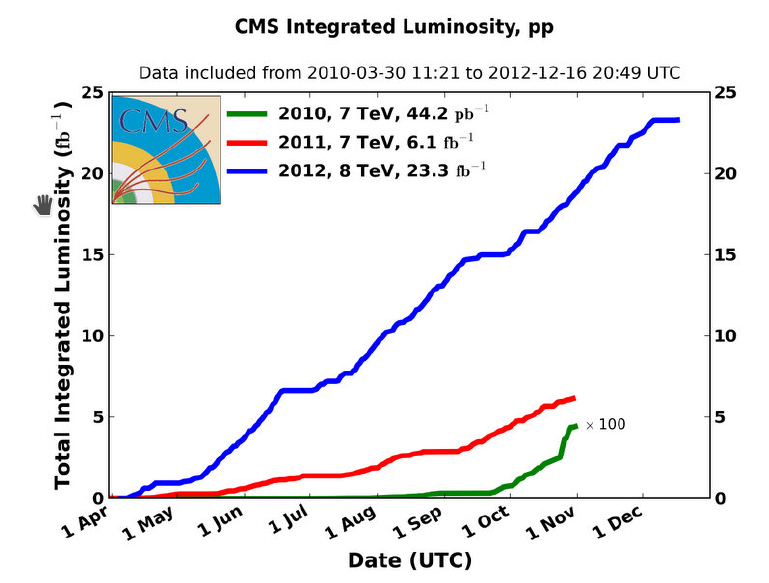
\includegraphics[height=5cm,width=7cm]{5}
		\caption{Integrated Luminosity at LHC RUN 1.}
	\end{figure}	
\end{frame}


% HHHHHHHHHHHHHHHHHHHHHHHHHHHHHHHHHHHHHHHHHHHHHHHHHHHHHHHHHHHHHHHHH

\section{Other experiments at LHC.}

% HHHHHHHHHHHHHHHHHHHHHHHHHHHHHHHHHHHHHHHHHHHHHHHHHHHHHHHHHHHHHHHHH

\begin{frame}[fragile]{ALICE.}
A Large Ion Collider Experiment is located at point 2 of the LHC main ring.

Designed for Heavy Ions Physics.
\\
\begin{minipage}{0.7\textwidth}% adapt widths of minipages to your needs
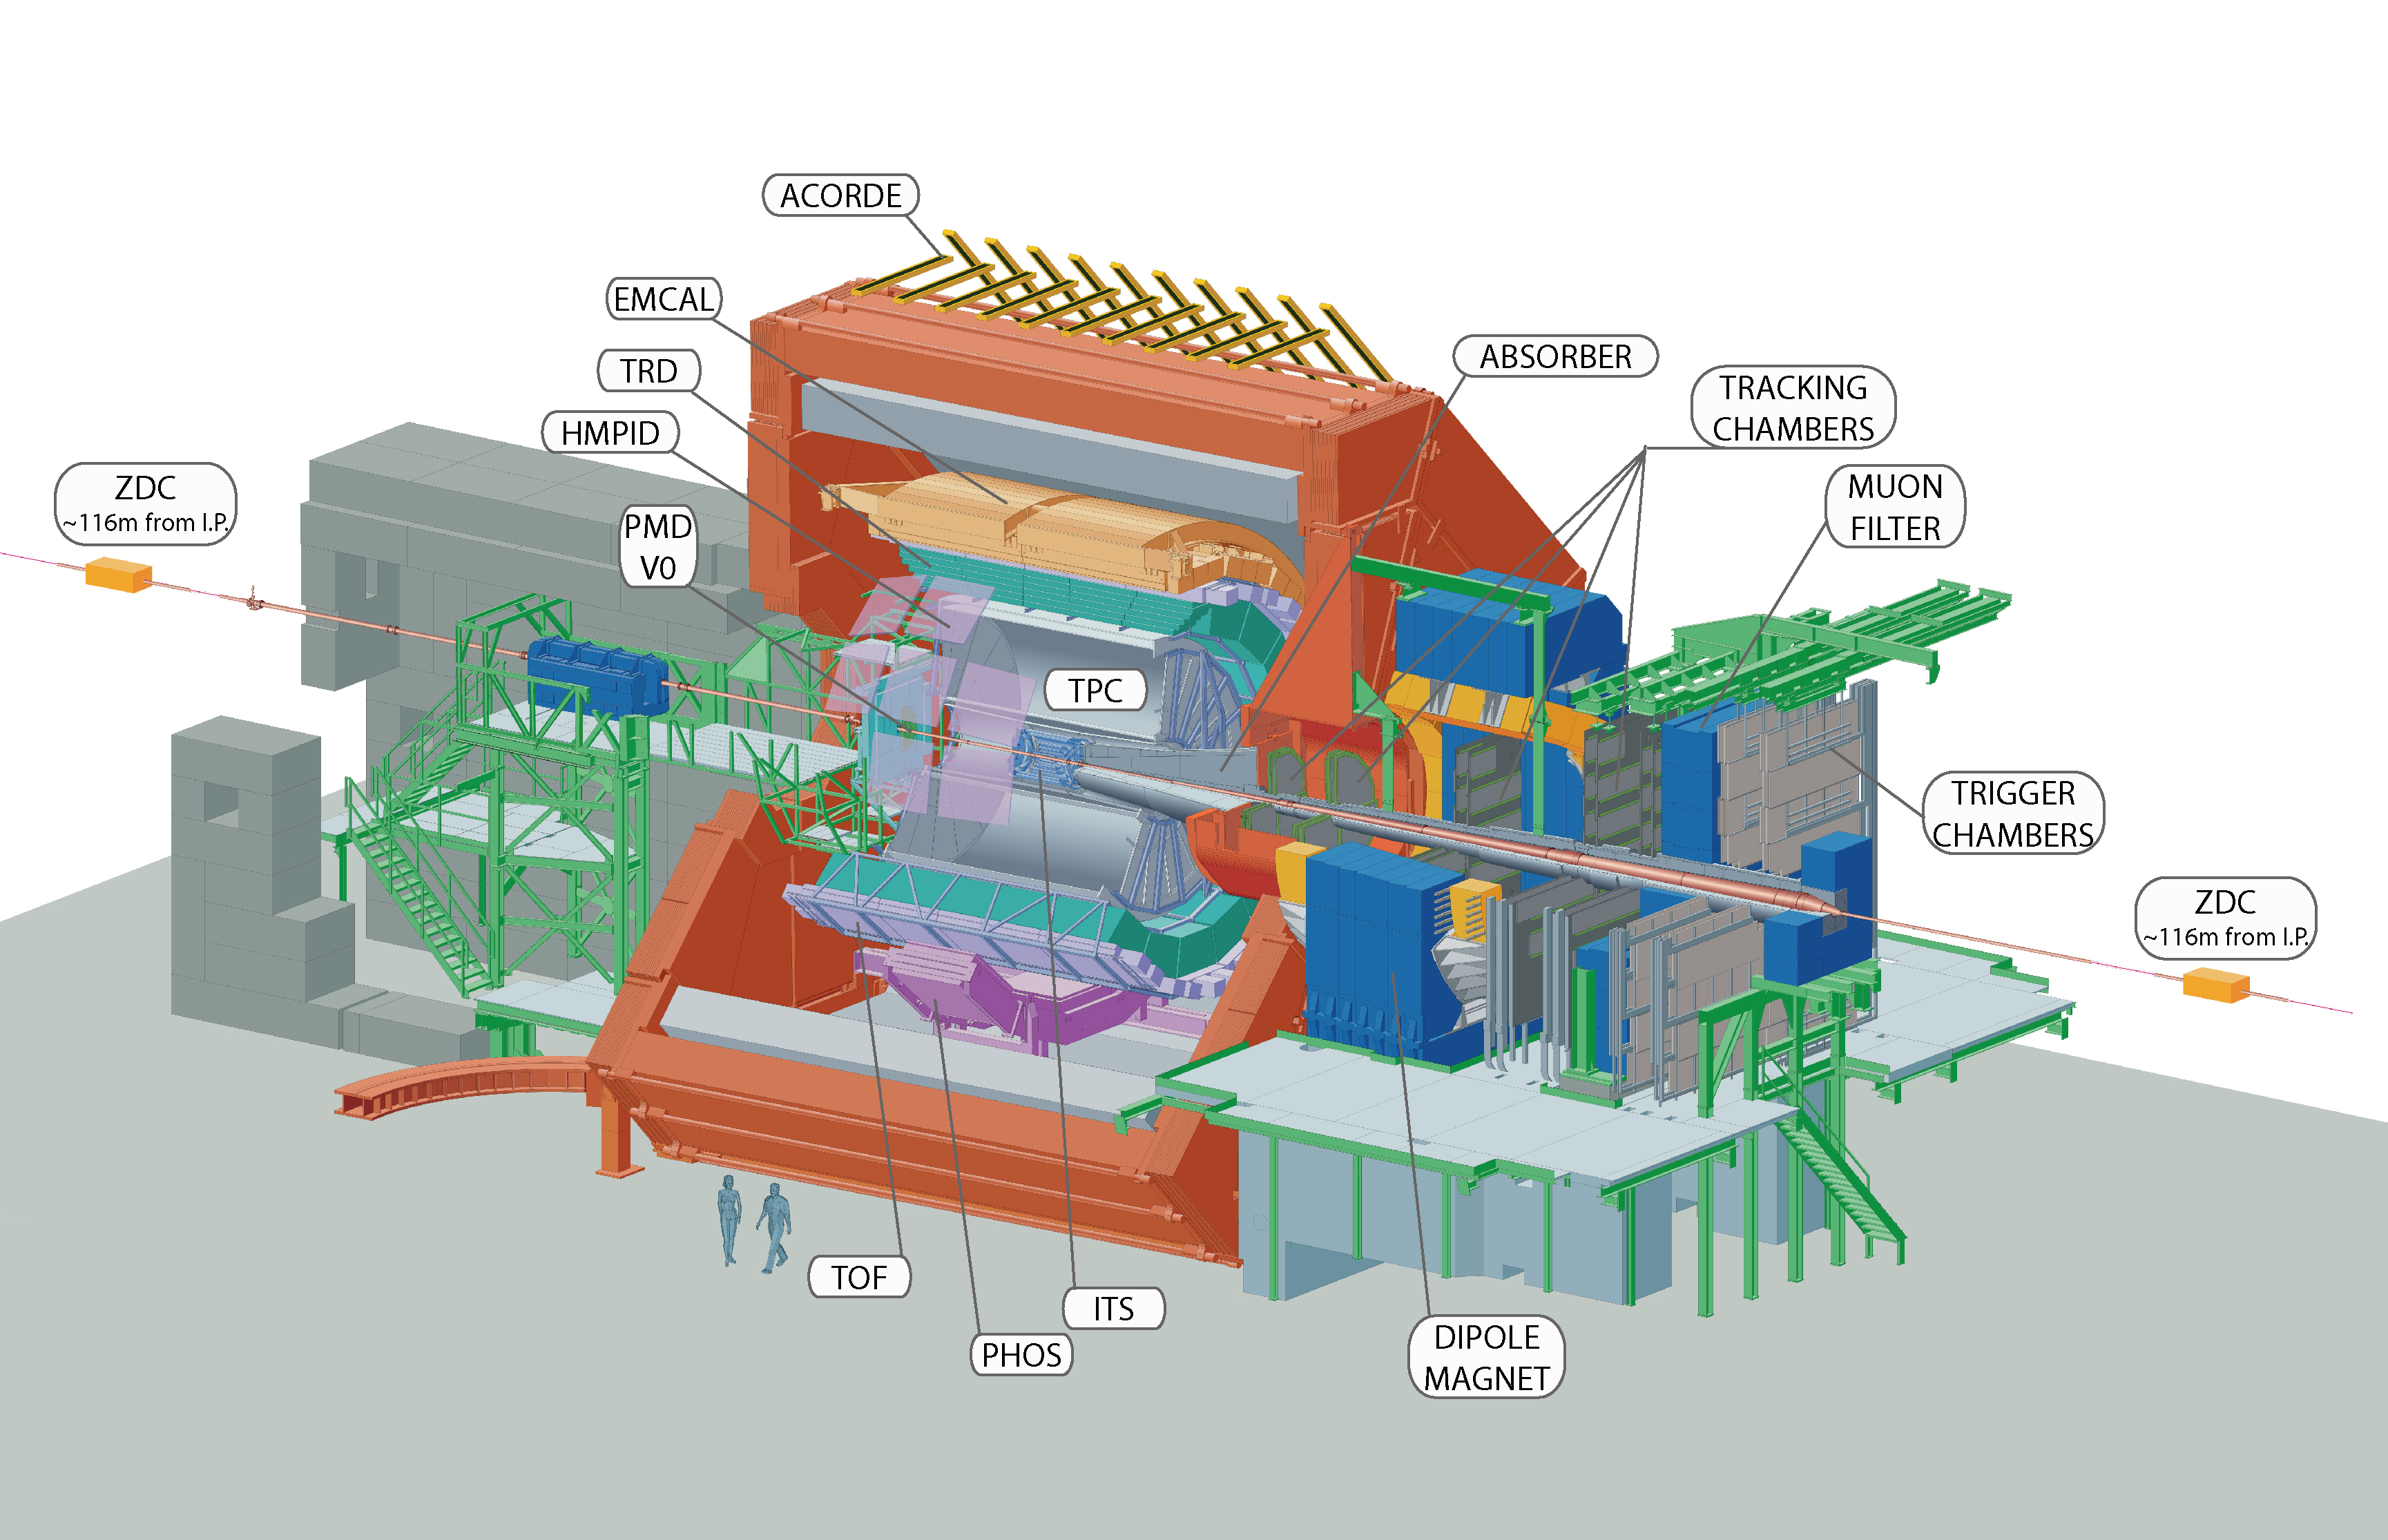
\includegraphics[width=7cm]{6}
\end{minipage}%
\hfill%
\begin{minipage}{0.3\textwidth}\raggedleft
	\begin{itemize}
		\item H=16m,W=16m,L=26m. Weight=10000 Tons.	
		\item Able to detect an extremely high number of tracks per event.
		\item Main subsystem: Time proyection chamber, a 90 $m^3$ gas chamber operated in a soleniod of 0.5T.
	\end{itemize}
\end{minipage}
\\
\vspace{0.5cm}

ALICE collaboration counts around 1500 people from 154 physics institutes in 37 countries.
\end{frame}

% HHHHHHHHHHHHHHHHHHHHHHHHHHHHHHHHHHHHHHHHHHHHHHHHHHHHHHHHHHHHHHHHH

\begin{frame}[fragile]{ATLAS.}
	A Toroidal LHC ApparatuS is the biggest LHC experiment, located at point 1.
	\vspace{0.5cm}
	\\
	\begin{minipage}{0.7\textwidth}% adapt widths of minipages to your needs
		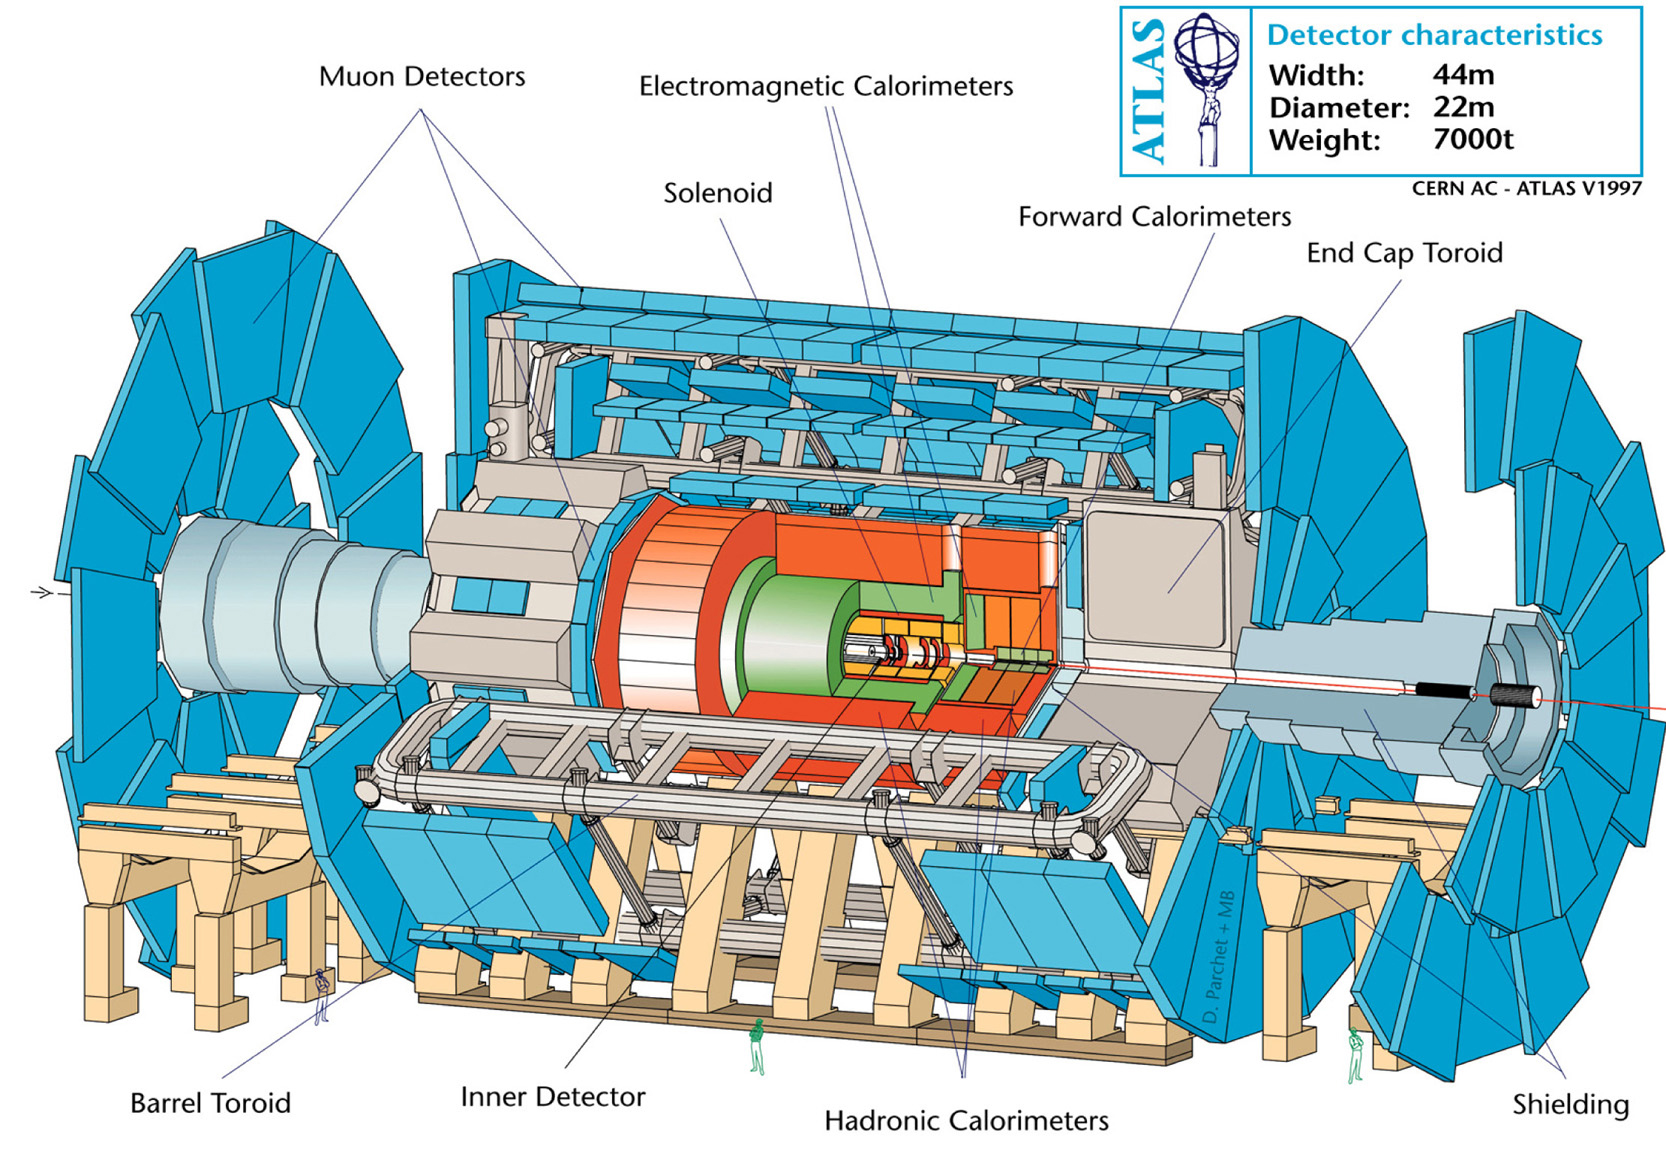
\includegraphics[width=7cm]{7}
	\end{minipage}%
	\hfill%
	\begin{minipage}{0.3\textwidth}\raggedleft
		\begin{itemize}
			\item H=25m,L=45m. Weight=7000 Tons.
			\\
			\vspace{0.5cm}
			Its main components are:	
			\item Tracker system.
			\item EM Calorimeter.
			\item Hadron calorimeter.
			\item Muon chambers.
		\end{itemize}
	\end{minipage}
	\\
	\vspace{0.5cm}
	ATLAS collaboration counts around 3000 people from 117 physics institutes in 38 countries.
\end{frame}

% HHHHHHHHHHHHHHHHHHHHHHHHHHHHHHHHHHHHHHHHHHHHHHHHHHHHHHHHHHHHHHHHH

\begin{frame}[fragile]{LHCb.}
	Located at point 8, it was designed to detect particles produced close to the beam direction.
	Smaller than CMS and ATLAS and conically shaped.

	\vspace{0.5cm}
	\begin{minipage}{0.7\textwidth}% adapt widths of minipages to your needs
		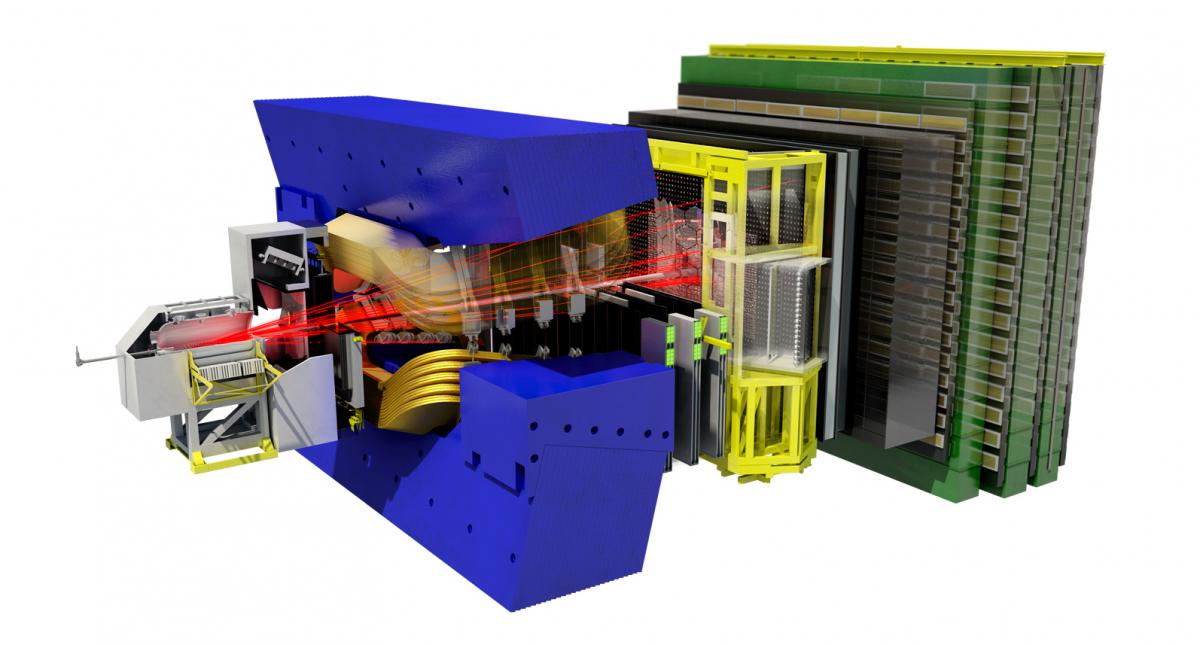
\includegraphics[width=7cm]{8}
	\end{minipage}%
	\hfill%
	\begin{minipage}{0.3\textwidth}\raggedleft
		\begin{itemize}
			\item H=10m,L=21m,W=13m. Weight=4500 Tons.		
			\item It has a system to detect different type of Hadrons.
			\item Very precise vertex locator system.
		
		\end{itemize}
	\end{minipage}
	\\
	\vspace{0.5cm}
	LHCb collaboration counts around 700 people from 69 physics institutes in 17 countries.
\end{frame}


\section{CMS.}

% HHHHHHHHHHHHHHHHHHHHHHHHHHHHHHHHHHHHHHHHHHHHHHHHHHHHHHHHHHHHHHHHH

\begin{frame}[fragile]{The Compact Muon Solenoid.}
	Located at point 5, its the second biggest LHC experiment, its called compact because the calorimeters are inside the magnet, and muon solenoid because it has a very precise muon detection system.
	
	\vspace{0.5cm}
	\begin{minipage}{0.7\textwidth}% adapt widths of minipages to your needs
		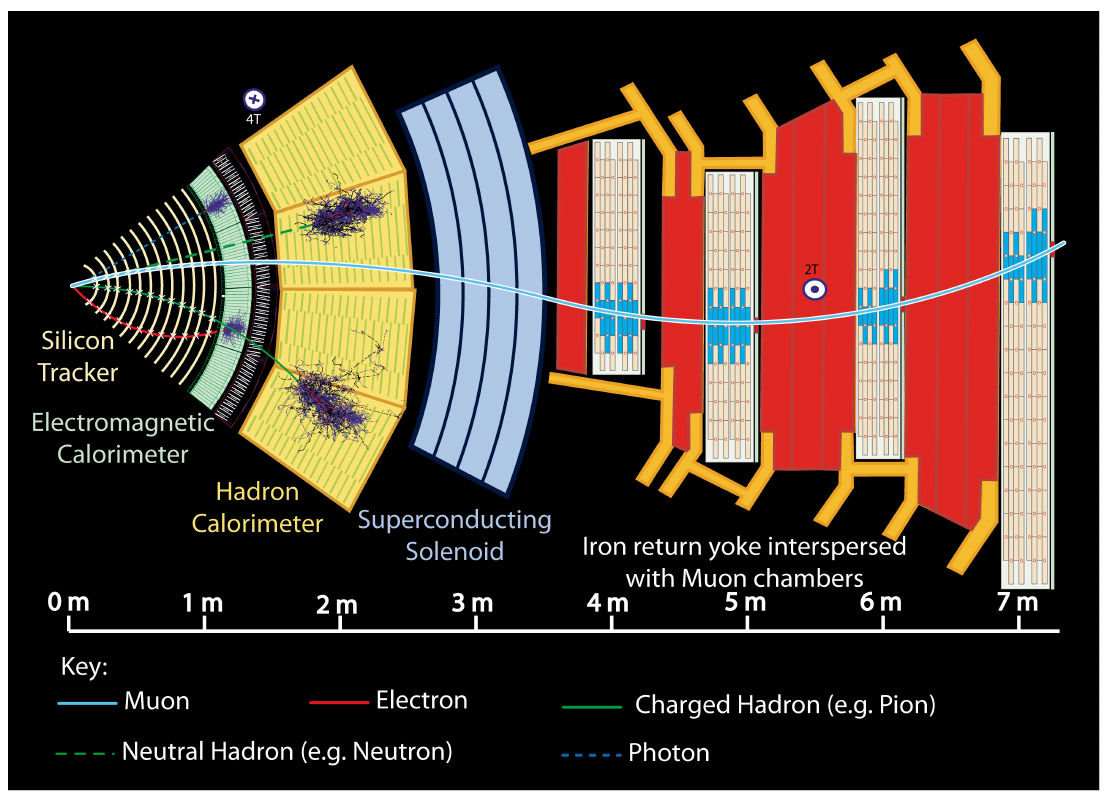
\includegraphics[width=7.5cm]{9}
	\end{minipage}%
	\hfill%
	\begin{minipage}{0.3\textwidth}\raggedleft
		\begin{itemize}
			\item H=15m,L=28.7m. Weight=14000 Tons.		
			\item 3.8T magnetic field.
			\item The energy of jets wit $p_T>20GeV/c$ can be measured with 4\% uncertainty.
			
		\end{itemize}
	\end{minipage}
	\\
	\vspace{0.5cm}
	CMS collaboration counts around 3500$+$3 people from 181$+$1 physics institutes in 41 countries.
\end{frame} 

% HHHHHHHHHHHHHHHHHHHHHHHHHHHHHHHHHHHHHHHHHHHHHHHHHHHHHHHHHHHHHHHHH

\begin{frame}[fragile]{Coordinate system.}
	The coordinate origin is located at the center of CMS, in the "iteraction point".
	\\
	Z axis: defined in the beam direction, poingting towards Jura mountains.
	\\
	Y axis: defined towards the zenit.
	X axis: pointing to the center of LHC ring.
	\\
	$\phi$ angle: Defined in x-y plane from x to y.
	$\theta$ angle: Located at z-y plane, from z to y.
	\vspace{0.5cm}
	\begin{minipage}{0.6\textwidth}% adapt widths of minipages to your needs
		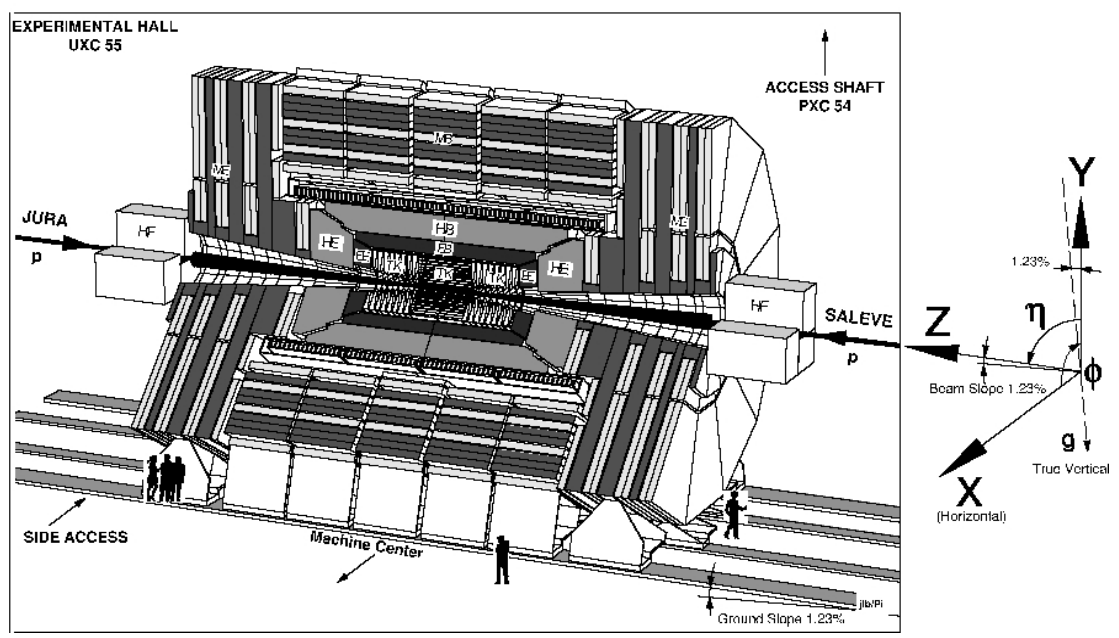
\includegraphics[width=7.5cm]{10}
	\end{minipage}
	\hfill
	\begin{minipage}{0.3\textwidth}\raggedleft
		\justify
		The commonly used momentum variables are:
		\\
		1. \textbf{$p_L$} Momenta in the z axis.
		\\
		2. \textbf{$p_T$} Momenta in te x-y plane.
		\\
		It is always preferable to use pseudorapidity instead of $\theta$:
		$\eta=-\log\tan\left(\frac{\theta}{2}\right)$
		
	\end{minipage}
	\textbf{Magnet}
	The CMS has a large solenoid capable of producing a 4T constant magnetic field inside the 6m diameter and 13m long magnet. It weights 12000 and is made of 4 Layers of windings of NbTi cable at 4.45K to achieve superconducting state.
	
	Outside the magnet 5 wheels and 3 disks of iron are placed to return the magnetic flux and inducing an external field of 2T.

\end{frame}

% HHHHHHHHHHHHHHHHHHHHHHHHHHHHHHHHHHHHHHHHHHHHHHHHHHHHHHHHHHHHHHHHH

\begin{frame}[fragile]{Tracker system.}
	Designed with two technologies: Pixels and Silicon strips, 
	the pixels have a cell size of 100*150 $\mu m^2$ and the system achieves a resolution of 9$\mu m$.
	\\
	The efficiency is higher than 98\% for all layer and disks, but it degrades with integrated luminosity.
	\\
	Designed to reconstruc high $p_T$ leptons and as consequence photons, it can reconstruct secondary vertexes and has an efficiency from 85 to 95\% for particles with $p_T$ between 0.1-10 GeV.
	\\ Constructed for being highly resistant to radiation, its expected to last for 10 years. 
	

		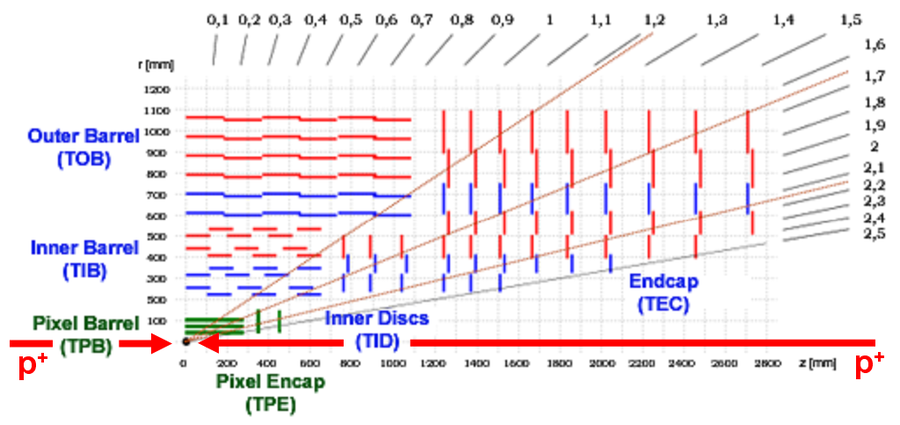
\includegraphics[width=10.5cm]{11}

\end{frame}

% HHHHHHHHHHHHHHHHHHHHHHHHHHHHHHHHHHHHHHHHHHHHHHHHHHHHHHHHHHHHHHHHH

\begin{frame}[fragile]{Tracker system.}
	
	
	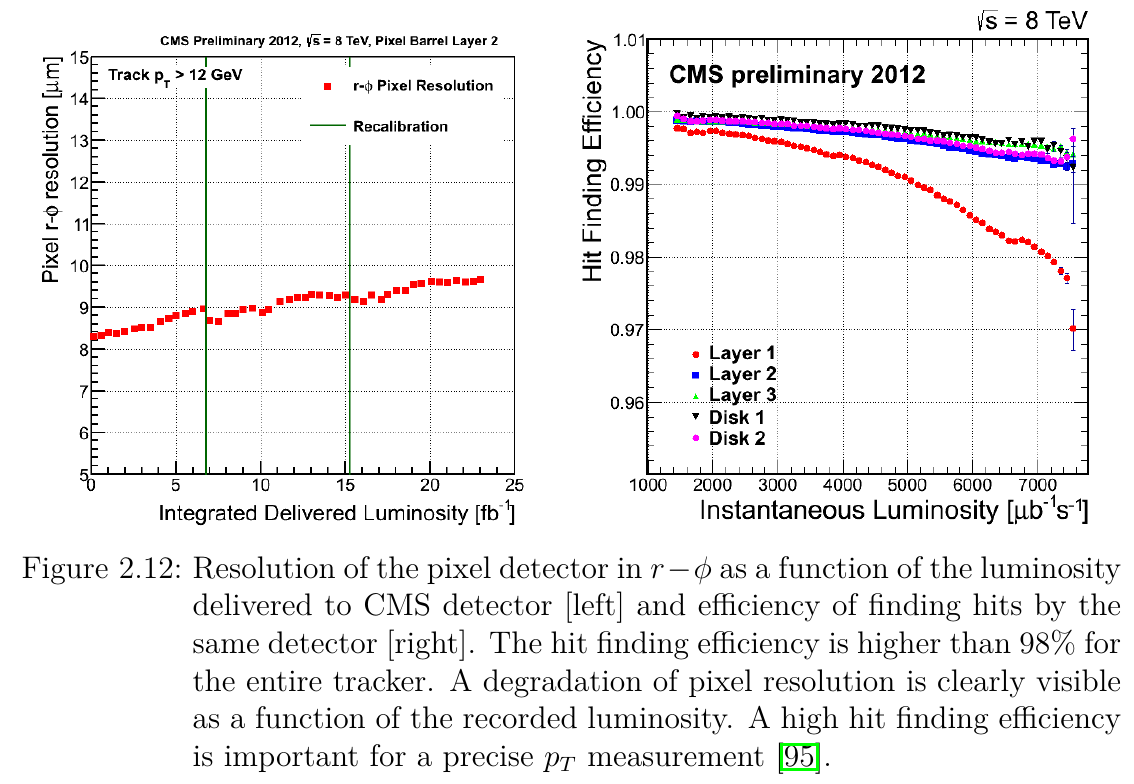
\includegraphics[width=10.5cm]{12}
	
\end{frame}


% HHHHHHHHHHHHHHHHHHHHHHHHHHHHHHHHHHHHHHHHHHHHHHHHHHHHHHHHHHHHHHHHH

\begin{frame}[fragile]{Electromagnetic Calorimeter.}
	The CMS ECAL system was designed to stop photons and electrons and measure their energy, it is a cylindrical hermetic calorimeter made of 61200 crystals in the barrel and 7324 in the endcap.\\
	The crystal material is lead tungstate and was chosen for its short radiation depth, high density and fast emitting scintillation (25 ns). Its main disadventage is its highly dependent response to temperature. (2\%/C)
	\\
	This systems need constant correction because it loss of transparency due to radiation, the crystals aging is calibrated by a laser system.
	\centering
	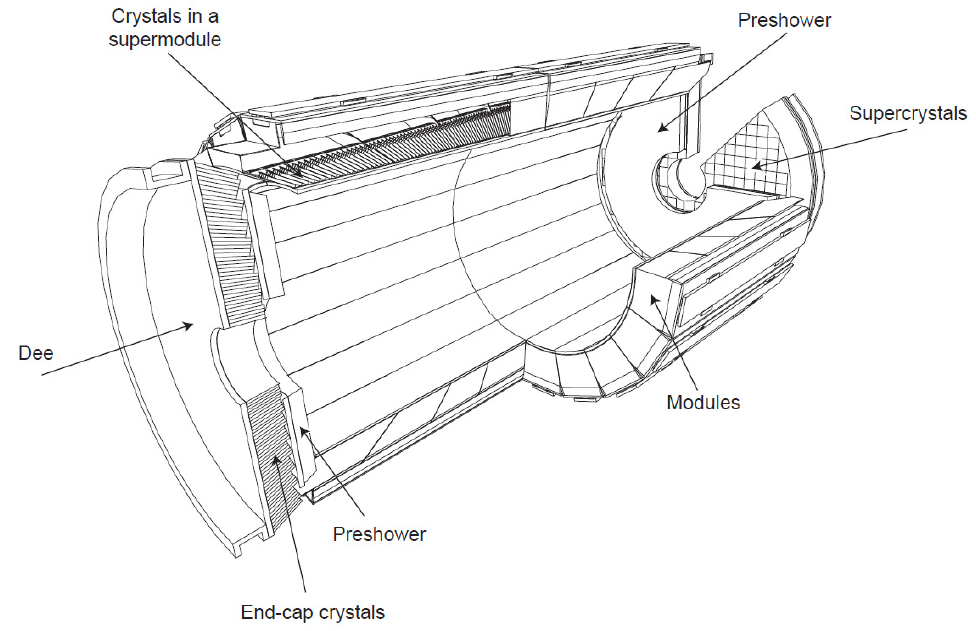
\includegraphics[width=8cm]{13}

\end{frame}

% HHHHHHHHHHHHHHHHHHHHHHHHHHHHHHHHHHHHHHHHHHHHHHHHHHHHHHHHHHHHHHHHH

\begin{frame}[fragile]{Electromagnetic Calorimeter.}
	
	\centering
	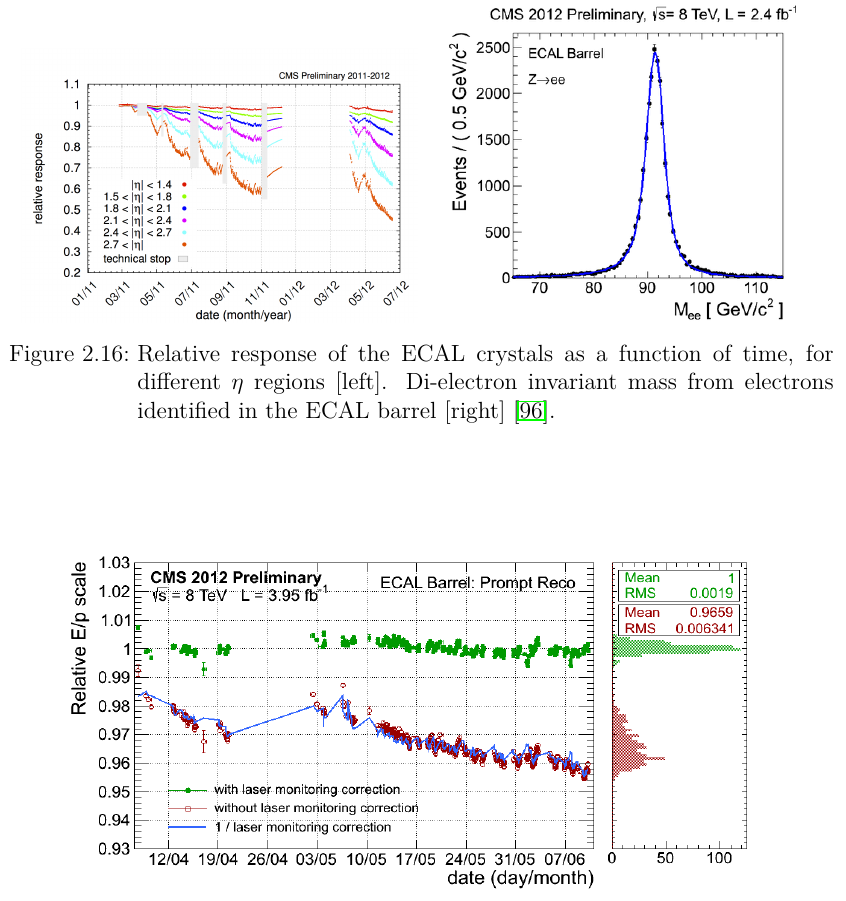
\includegraphics[width=8cm]{14}
	
\end{frame}


% HHHHHHHHHHHHHHHHHHHHHHHHHHHHHHHHHHHHHHHHHHHHHHHHHHHHHHHHHHHHHHHHH

\begin{frame}[fragile]{Hadronic Calorimeter.}
	The CMS HCAL is the subsystem made for hadron detection, its subdivided as:
	\begin{itemize}
		\item Hadron Barrel Calorimeter (HB): Covering $|\eta| < 1.4$ is located between the	ECAL barrel and the magnet.
		\item Hadron Endcap Calorimeter (HE): Extends the coverage of the barrel in the
		region $1.4 <|\eta| < 3$.
		\item Hadron Outer Calorimeter (HO): Located outside the magnet.
		\item Hadron Forward Calorimeter (HF): Completes the coverage of the system
		from $|\eta| = 3$ up to $|\eta| = 5.2$.
	\end{itemize}
	
	
	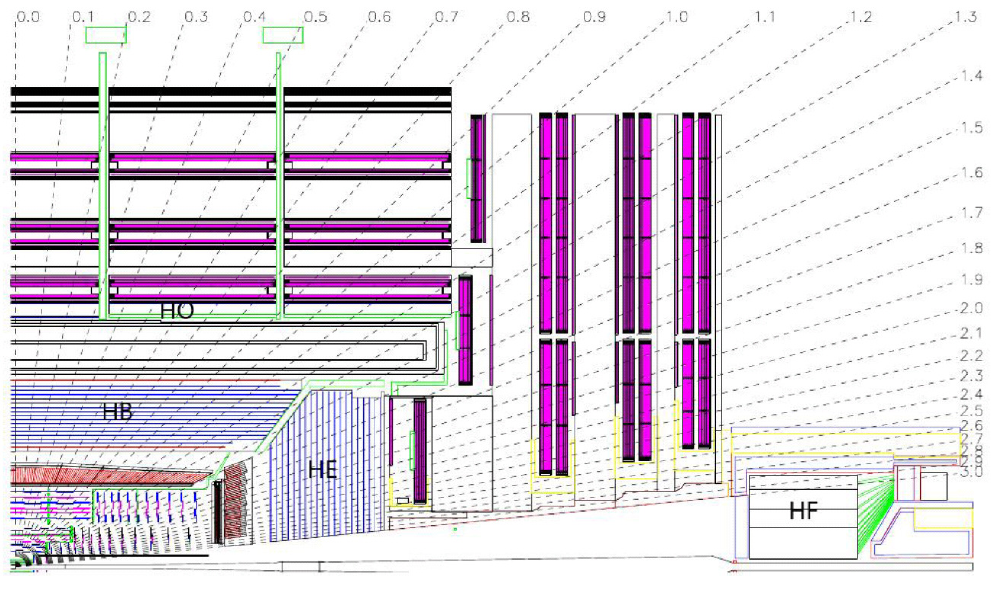
\includegraphics[width=9cm]{15}
\end{frame}

% HHHHHHHHHHHHHHHHHHHHHHHHHHHHHHHHHHHHHHHHHHHHHHHHHHHHHHHHHHHHHHHHH

\begin{frame}[fragile]{Hadronic Calorimeter.}
	The system is made of two parts: absorbers to develop hadronic showers and scintillators to measure particles energy. 
	\\
	The HB absorber	is made of 40 mm thick steel plate, 8 layers of brass plates of 50.5 mm , 6 brass plates of 56.5 mm and a steel plate of 75 mm . The HE	uses the same absorber but with thicker plates of 79 mm. Between the absorber	plates a plastic scintillator, Kuraray SCSN81, 3.7 mm thick, is placed.
	\\
	\metroset{block=fill}
	\begin{exampleblock}{}
		The produced light in the HB is collected by optical fibers and
		transferred to the Hybrid Photo Diodes (HPDs). These diodes were chosen because
		of their small sensitivity to the magnetic field, an important feature because HCAL
		is inside the solenoid magnet.
		
	\end{exampleblock}
	
	\metroset{block=fill}
	\begin{exampleblock}{High radiation problem at HF}
		The HF design is different from the rest of the HCAL . The most
		important challengeis the high resistance to radiation from collisions:
		while in the central rapidity region, 100 GeV are deposited in average, in the
		forward region, is 760 GeV. For this reason a Cherenkov detector made of quartz fibers with a steel absorber was chosen. The light produced in the
		HF is collected by photo multipliers.
		
	\end{exampleblock}

	
\end{frame}



% HHHHHHHHHHHHHHHHHHHHHHHHHHHHHHHHHHHHHHHHHHHHHHHHHHHHHHHHHHHHHHHHH
\begin{frame}[fragile]{Muon Chambers.}
	The muon detector systems is located at the most exterior layer of the dectector due to the high prenetration power of muons. The cambers are made of three subsystems:
	

		\begin{itemize}
			\item  Drift Tubes Chambers (DT): located in the region with $ |\eta|< 1.2$ and disposed in four layers. They consist of individual drift tubes of 50 $\mu$m of diameter anode wire with two electrode plates creating a drift electric field.
			The wall of the cell act as cathode. The cells are filled with a gas mixture,
			85\% Argon and 15\% CO2 .
			
						
			\item  Cathode Strip Chambers (CSC): installed in the endcaps, provide a coverage up to $|\eta| = 2.4$ from $|\eta| = 0.9$. These chambers are multi-wire proportional chambers made of six planes of anode wires with 7 cathode planes with a gas in the middle and perpendicular to each other. This system is able to measure with a precision between the 75 $\mu$m and 150 $\mu$m.
			\item  Resistive Plate Chambers (RPC): This subsystem is made of gaseous parallel plate detectors. This detector is specially useful for triggering as it is very fast and have a good position resolution. There are 480 RPC distributed in	6 layers in the barrel with the DT and in 3 layers in the endcaps with the CSC, and covers the region with$|\eta|  < 1.6$.
			
		\end{itemize}
		
		
\end{frame}

% HHHHHHHHHHHHHHHHHHHHHHHHHHHHHHHHHHHHHHHHHHHHHHHHHHHHHHHHHHHHHHHHH
\begin{frame}[fragile]{Muon Chambers.}
	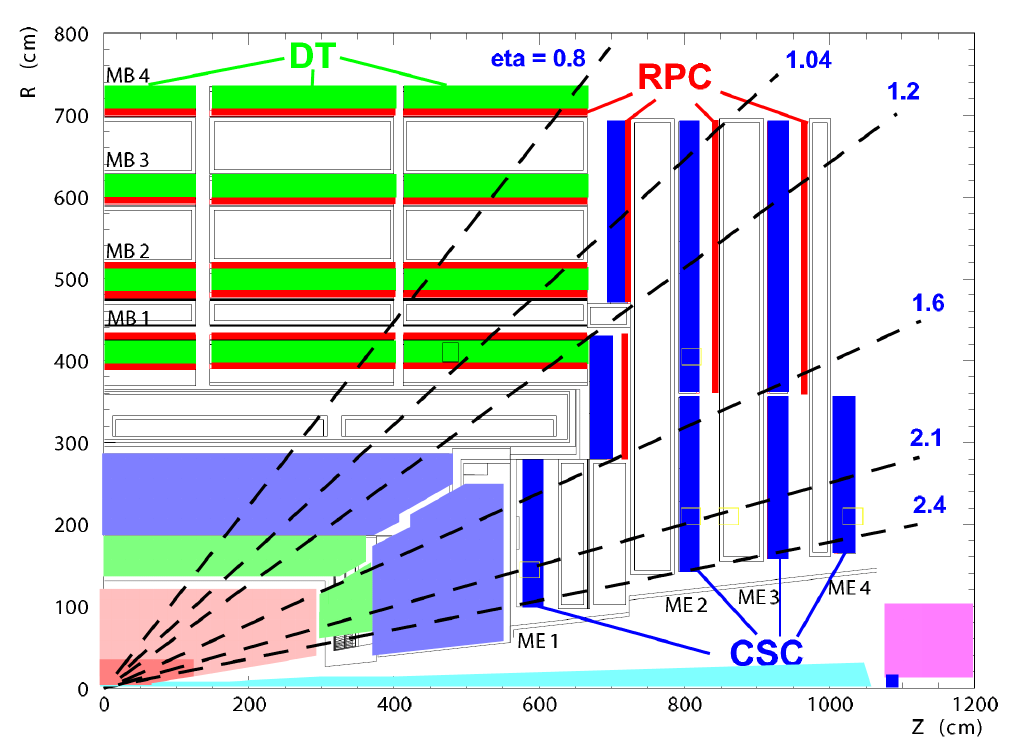
\includegraphics[width=11cm]{16}
\end{frame}
% HHHHHHHHHHHHHHHHHHHHHHHHHHHHHHHHHHHHHHHHHHHHHHHHHHHHHHHHHHHHHHHHH
\begin{frame}[fragile]{Trigger.}
	LHC was designed to collect data from collisions every 25 ns, each single event produces 0.5-1 MB of information thus the total data flow is 1PB/s.	An on-line selection must be done, the trigger system of CMS does the job in two stages: 
		\metroset{block=fill}
		\begin{exampleblock}{Level 1 trigger (L1)}
			\begin{itemize}
				\item Hardware based, it reduces the data flow by 2 order of magnitude. It is an extremely fast and wholly automatic process that looks for simple signs of interesting physics, e.g. particles with a large amount of energy or in unusual combinations.
				\item The latency time that the L1 disposes between the
				collision and the taking of the decision is about 3.2 $\mu$s. Therefore, the front-end
				memory in the cards should be able to keep in memory up to 128 bunch crossings.
			\end{itemize}

			
		\end{exampleblock}
			\metroset{block=fill}
			\begin{exampleblock}{High level trigger (HLT)}
				\begin{itemize}
					\item 	A set of filtering algorithms that run in CPU farms of about $10^4$ cores. 
					\item During 2012, the decision taking process was 110 ms, around $10^5$ times more than for the L1.
					\item  There is a constant development of HLT paths focusing on different analysis requirements in order to obtain the best possible selection efficiency for specific signal types.
					
				\end{itemize}
				
			
				
				
			\end{exampleblock}
\end{frame}


\section{Conclusions.}


% HHHHHHHHHHHHHHHHHHHHHHHHHHHHHHHHHHHHHHHHHHHHHHHHHHHHHHHHHHHHHHHHH
\begin{frame}[fragile]{Conclusions.}

		\begin{itemize}
			\item CMS has an extremely precise quantity of systems capable of detecting electrons, photons, hadrons and muons, reconstructing vertices, tracks and energy for this kind of particles.
			\item Systems like the ECAL, HCAL and Tracker have to be recalibrated constantly because of the damage make to its subsystems by radiation 
			\item Due to the big amount of data produced every second by the collisions , data has to be selected in an on-line process, the CMS Trigger system does this job reducing the data flow by $10^5$ orders of magnitude. 
			\item CMS detector is an incredibly complex experiment and its important for experimental particle physicists to know how this detector works in order to know how and where to search for new physics.
		\end{itemize}
		
		
	
\end{frame}


% HHHHHHHHHHHHHHHHHHHHHHHHHHHHHHHHHHHHHHHHHHHHHHHHHHHHHHHHHHHHHHHHH
\begin{frame}[fragile]{Bibliography.}
	
	\begin{itemize}
		\item Search for a vector-like quark T decaying
		into top$+$Higgs in single production mode
		in full hadronic final state using
		CMS data collected at 8 TeV, José David Ruiz.
		
		\item Concept of Luminosity, Werner Herr and Bruno Muratori.
		\item Study of the inclusive beauty production at CMS and construction and comissioning of the CMS pixel barrel detector, Caminada,L.
		\item https://cms.cern/detector.
	\end{itemize}
	
	
	
\end{frame}

\end{document}

